
\begin{questions}

% 3.2  % % % % % % % % % % % % % % % % % % % % %
\setcounter{question}{1}
\question{
Seja $f \, : \, \R^2 \setminus \{ (0,0) \} \longrightarrow \R$ a função dada por
\[
f(x,y) = \frac{xy^2}{x^2 + y^4}.
\]
Mostre que $\displaystyle\lim_{(x,y) \to (0,0)} f(x,y)$ não existe.
}
\begin{solution}
    Tome o caminho $x = y^2$, então
    \[
        \lim_{y\to 0} f(y^2,y) = \lim_{y\to 0} \frac{y^4}{y^4+y^4} = \frac{1}{2}.
    \]
    Porém, com o caminho $x=y$, temos que
    \[
        \lim_{y\to 0} f(y,y) = \lim_{y\to 0} \frac{y^3}{y^2+y^4} = \lim_{y\to 0} \frac{y}{1+y^2} = 0.
    \]
    Portanto, o limite $\displaystyle\lim_{(x,y) \to (0,0)} f(x,y)$ não existe, pois resulta em diferentes valores para diferentes caminhos.
\end{solution}

% 3.3 % % % % % % % % % % % % % % % % % % % % %
% \setcounter{question}{2}
\question{
Calcule o limite
\[
\lim_{(x,y) \to (0,0)} \frac{x^2 y}{x^2 + y^2},
\]
se este existir. Se a existência for confirmada, que valor devemos arbitrar para a função $f \, : \, \R^2 \setminus \{ (0,0) \} \longrightarrow \R$ dada por $f(x,y) = \frac{x^2 y}{x^2 + y^2}$ para que $f$ seja contínua?
}

\begin{solution}
    Vamos re-escrever o limite em coordenadas polares, ou seja,
    \[
        \lim_{(x,y) \to (0,0)} \frac{x^2 y}{x^2 + y^2}
            = \lim_{r \to 0^+} \frac{r^2\cos^2(\theta)\,r \sin(\theta)}{r^2}
            = \lim_{r \to 0^+} r \cos^2\theta \sin \theta.
    \]
    Sabemos que
    $
    -|r| \le r \cos^2\theta \sin \theta \le |r|.
    $
    Portanto, podemos concluir através do Teorema do Confronto que o limite que desejamos calcular existe e é nulo.
    
    Dessa forma, $f$ é contínua em $\R^2$ se definida da seguinte forma
    \[
    f(x,y) =
    \begin{cases}
        \frac{x^2 y}{x^2 + y^2}, &\text{se }(x,y)\neq(0,0),\\
        0,  &\text{se }(x,y)=(0,0).
    \end{cases}
    \]
\end{solution}

% 3.7 % % % % % % % % % % % % % % % % % % % % %
\setcounter{question}{6}
\question{
Encontre os pontos do elipsóide $x^2 + 2y^2 + 3z^2 = 1$ em que o plano tangente é paralelo ao plano $3x - y + 3z = 1$. 
}

\begin{solution}
    Sejam duas superfícies de nível $\cal{S}_1 = \{\vec r\in \R^3 : f_1(\vec r) = c_1 \}$, $\cal{S}_2 = \{\vec r \in \R^3 : f_2(\vec r) = c_2 \}$, $f_1,f_2: \R^3 \longrightarrow \R$.
    %
    Sabemos que planos tangentes às superfícies nos pontos $\vec r_1\in\cal{S}_1$ e $\vec r_2 \in \cal{S}_2$ são paralelos sempre que
    $
        \nabla f_1(\vec r_1) = \alpha \nabla f_2(\vec r_2)
    $
    para algum $\alpha\in\R^*$.
    
    Para o nosso problema, temos que
    \[
        (2x, 4y, 6z) = \alpha\,(3,-1,3)
            ~ \Rightarrow (x,y,z) = \alpha\,(3/2,-1/4,1/2).
    \]
    Substituindo na equação do elipsoide temos que
    \[
        \left( \frac{3}{2} \alpha \right)^2+2\left( \frac{1}{4} \alpha\right)^2+3\left( \frac{1}{2} \alpha\right)^2 = 1
            ~ \Rightarrow \alpha = \pm\frac{2\sqrt{2}}{5}.
    \]
    Portanto, os pontos do elipsoide são $\pm\frac{\sqrt{2}}{10}\left(6,-1,2\right)$.
\end{solution}

% 3.9 % % % % % % % % % % % % % % % % % % % % %
\setcounter{question}{8}
\question{
Calcule o volume do sólido definido pelo parabolóide $x^2/4 + y^2/9 + z = 1$ e pelo quadrado $R = [-1,1]\times[-2,2]$ no plano $z = 0$.
}

\begin{solution}
    \begin{align*}
        \int_{1}^{2} \int_{-2}^{-1} \int_{0}^{1-x^2/4-y^2/9} \mathrm{d}z\,\mathrm{d}x\,\mathrm{d}y = \frac{17}{108}.
    \end{align*}
\end{solution}

% 3.10 % % % % % % % % % % % % % % % % % % % % %
% \setcounter{question}{5}
\question{
Encontre o volume do sólido delimitado pelos cilindros $x^2 + z^2 = r^2$ e $y^2 + z^2 = r^2$.
}

\begin{solution}
    ~
    \begin{center}
        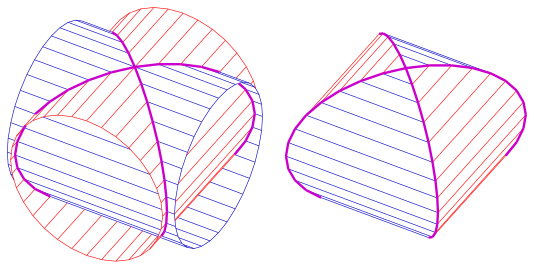
\includegraphics[width=0.5\paperwidth]{ex_3-10.png}
    \end{center}
    Note que a a região a ser integrada é formada por chapas quadradas de lado $2\sqrt{r^2-z^2}$.
    \begin{align*}
        V = \int_{-r}^r \int_{-\sqrt{r^2-z^2}}^{\sqrt{r^2-z^2}} \int_{-\sqrt{r^2-z^2}}^{\sqrt{r^2-z^2}} \diff x\,\diff y\,\diff z
            = \int_{-r}^r 4\,(r^2-z^2)\,\diff z
            = \frac{16}{3} r^3.
    \end{align*}
    
\end{solution}


% 3.11  % % % % % % % % % % % % % % % % % % % % %
% \setcounter{question}{7}
\question{
Calcule o volume do sólido delimitado inferiormente pelo cone $z = \sqrt{x^2 + y^2}$ e superiormente pela esfera $x^2 + y^2 + z^2 = 1$.
}

\begin{solution}
    Em coordenadas cilíndricas temos que o volume
    \begin{align*}
        V = \int_{0}^{\sqrt{2}/2}\int_{r}^{\sqrt{1-r^2}}\int_{0}^{2\pi} r\,\diff \theta\,\diff z\,\diff r
            = 2\pi \int_{0}^{\sqrt{2}/2} \left( r\sqrt{1-r^2} - r^2 \right) \diff r
            = \left(2-\sqrt{2}\right) \frac{\pi}{3}.
    \end{align*}
    Note que o limite de integração $0 \le r \le \sqrt{2}/2$ se deve ao fato que a esfera intersecta o cilindro em $r^2+r^2=1$, ou seja, em $r = \sqrt{2}/2$.
\end{solution}

% 3.12 % % % % % % % % % % % % % % % % % % % % %
% \setcounter{question}{5}
\question{
Calcule o volume do sólido delimitado superiormente pelo plano $z = 4$, inferiormente pelo parabolóide $z = 1 - x^2 - y^2$ e lateralmente pelo cilindro $x^2 + y^2 = 1$.
}

\begin{solution}
    Em coordenadas cilíndricas temos que o volume
    \begin{align*}
        V = \int_{0}^{1} \int_{1-r^2}^{4}\int_{0}^{2\pi} r\,\diff \theta\,\diff z\,\diff r
            = 2\pi \int_{0}^{1} \left( 3r+r^3 \right) \diff r
            = \frac{7\pi}{2}.
    \end{align*}
\end{solution}

\end{questions}
